% !TeX program = xelatex
% !BIB program = bibtex
% !TeX encoding = UTF-8
\documentclass[preprint,12pt]{elsarticle}

\ifdefined\synctex
  \synctex=1
\fi

\usepackage{amssymb}
\usepackage{amsmath}
\usepackage[a4paper,margin=1in]{geometry}
\usepackage{graphicx}
\usepackage{booktabs}
\usepackage{subcaption}
\usepackage{caption}
\usepackage{float}
\usepackage{algorithm}
\usepackage{algpseudocode}
\usepackage{multirow}
\usepackage{array}
\usepackage{enumitem}
\usepackage{needspace}
\usepackage[hidelinks]{hyperref}
\hypersetup{pdfauthor={},pdfsubject={},pdfkeywords={}}
\usepackage{fontspec}
\usepackage{xeCJK}
\setCJKmainfont{SimSun}

\graphicspath{{../05_figures/}}
\journal{Engineering Applications of Artificial Intelligence}

\setcounter{topnumber}{3}
\setcounter{bottomnumber}{2}
\setcounter{totalnumber}{5}
\renewcommand{\topfraction}{0.9}
\renewcommand{\bottomfraction}{0.8}
\renewcommand{\textfraction}{0.07}
\renewcommand{\floatpagefraction}{0.8}

\renewcommand{\algorithmicrequire}{\textbf{Require:}}
\renewcommand{\algorithmicensure}{\textbf{Ensure:}}

\captionsetup[figure]{name=Fig.}
\captionsetup[table]{name=Tab.}

\newcommand{\figref}[1]{Fig.\nobreakspace\ref{#1}}
\newcommand{\tabref}[1]{Tab.\nobreakspace\ref{#1}}

\begin{document}

\begin{frontmatter}

\title{Reinforcement Learning-Based Computer Numerical Control Motion Planning with Adaptive Preview and Jerk-Constrained Action Projection}

\begin{abstract}
Computer numerical control (CNC) motion planning converts computer-aided manufacturing (CAM)-generated tool paths into executable interpolation trajectories that satisfy contour tolerance and kinematic limits. Conventional smooth-then-schedule pipelines determine the geometric path before regulating the feedrate. After the path has been fixed, the feedrate planner can no longer use the tolerance band to adjust motion at corners and curvature-transition regions. This separation reduces the coupling between geometric smoothing and dynamic feasibility. We propose the Jerk-constrained Neural Numerical Controller (J-NNC), a closed-loop reinforcement learning framework that treats tolerance-band trajectory shaping and feedrate regulation as one constrained decision problem. Rather than selecting a path and then assigning its timing, J-NNC learns local motion decisions within the tolerance band and projects them onto the kinematically feasible set through a kinematic constraint module (KCM), thereby linking geometric freedom with jerk-limited execution. Experiments on square, circular, and butterfly-shaped paths show that J-NNC completes all cases with full path progress and no linear-jerk limit exceedance. It removes the violations observed in the neural-network numerical control (NNC) baseline and the no-KCM ablation. Compared with a traditional two-step baseline, J-NNC achieves a shorter execution time, a higher active jerk-limit engagement rate, and more effective use of the tolerance band while preserving jerk feasibility.
\end{abstract}

\begin{keyword}
computer numerical control \sep reinforcement learning \sep Adaptive Preview \sep jerk-constrained action projection
\end{keyword}

\end{frontmatter}

\section{Introduction}
\label{sec:introduction}
Conventional CNC motion planning usually follows a serial pipeline: the tool path is smoothed first, and feedrate planning is then carried out along the smoothed path~\cite{Sun2022,Yan2023}. This procedure improves the geometric continuity of CAM-generated tool paths. Once the smoothed trajectory is fixed, however, the feedrate planner can mainly adjust the motion speed along that trajectory~\cite{Erkorkmaz2001,Lee2011}. It has little room to reuse the spatial freedom inside the contour-tolerance band, especially in corner regions and curvature-transition regions~\cite{Sencer2015,Tajima2016}. For this reason, geometric smoothness, feedrate efficiency, and kinematic feasibility under velocity, acceleration, and jerk limits are difficult to optimize together in high-precision, high-speed machining~\cite{Sun2022,Zhang2021}.

In practice, this serial pipeline is built mainly from local smoothing, global smoothing, and feedrate scheduling. Local smoothing constructs transition curves between adjacent blocks. It is well suited to real-time interpolation because the computation is local and the contour error can be bounded explicitly~\cite{Hu2024}. Higher-order B\'ezier, B-spline, and curvature-smooth transitions can further improve acceleration or jerk continuity around corners~\cite{Fan2015,Zhang2018}. Dense short segments and consecutive corners, however, often leave only a limited transition length~\cite{Li2020}. Global smoothing reconstructs several segments over a larger domain and improves continuity for dense short-block paths~\cite{Song2021}. Under strict contour-error constraints, however, computational cost, iterative fitting, local feature preservation, and real-time implementation remain difficult~\cite{Yang2015}. Feedrate scheduling imposes velocity, acceleration, and jerk bounds along a selected path, but it usually starts from a predetermined geometric trajectory~\cite{Zhang2021}. NURBS and S-shaped schemes improve feasibility under chord-error and axial-drive constraints~\cite{Wu2022}. Look-ahead interpolation uses upcoming path information to regulate feedrate over short-line or spline tool paths~\cite{Tsai2010,Song2020}. These studies provide the main technical basis of the conventional serial CNC motion-planning pipeline.

Although this line of work has made substantial progress, the serial decomposition still separates geometry selection from timing regulation, even though these two decisions are physically coupled during interpolation. Local and global smoothing first determine the geometric curve used inside the contour-tolerance band, including the corner-transition shape and the curvature distribution. Feedrate scheduling then assigns a speed profile to the selected curve. The later stage can reduce or increase the feedrate, but it has limited ability to change how the tolerance band is used geometrically. This separation is especially restrictive when short segments, consecutive corners, and rapidly varying curvature appear in the same CAM path~\cite{Li2020,Zhao2013}. A conservative smoothing result may cause unnecessary deceleration, while an aggressive transition may still require speed reduction to satisfy acceleration or jerk limits~\cite{Sencer2015,Tajima2016}. Thus, a fixed serial procedure leaves limited room to balance the geometric use of the tolerance band with jerk-limited executable motion~\cite{Sun2022,Zhang2021}.

To address the limitations of the conventional serial pipeline, one-step methods aim to perform trajectory smoothing and feedrate planning within a unified planning process. Direct axis-velocity blending and integrated acceleration/deceleration interpolation plan axis motion near corners under real-time constraints~\cite{Tajima2016,Tsai2016}. Minimum-time cornering and high-speed cornering with vibration suppression optimize corner traversal under contour-error and actuator limits~\cite{Sencer2015,Duan2016}. Driving-force-constrained smoothing brings drive capability into corner planning, and quadratic B-spline fitting combines tool-path construction with optimal velocity interpolation under bounded error~\cite{Yang2015,LiDriving2017}. Integrated smoothing methods for line--arc and five-axis paths further handle transition overlap and feedrate fluctuation within unified smoothing procedures~\cite{Li2023,Sun2024}. In a closely related direction, Li et al. proposed neural-network numerical control (NNC), which treats CNC trajectory smoothing as a closed-loop action-decision problem and directly generates angle-change and step-length-change commands at each interpolation cycle~\cite{Li2020}. NNC shows that trajectory generation inside the tolerance band can be learned as an online decision process, with higher machining efficiency than local smoothing and higher contour accuracy than global smoothing~\cite{Li2020}.

These one-step methods strengthen the connection between path geometry and speed behavior, but several issues remain for tolerance-band CNC motion planning. Many optimization-based methods rely on predefined transition forms, local corner models, nonlinear constraints, or iterative computation. Their performance can therefore be sensitive to segment length, corner distribution, and local geometry variation~\cite{Yang2015,Li2023}. In NNC, the neural-network action is converted directly into an interpolation position or a servo command. If velocity, acceleration, and jerk constraints are not handled explicitly, or if no projection is applied at the execution layer, the generated command may violate the kinematic limits of the machine tool~\cite{Li2020}. In addition, the reward design mainly focuses on contour error, while path progress, direction consistency, motion smoothness, and stage-dependent behavior near corners receive less attention~\cite{Li2020}. These limitations make it difficult for one-step planning to use the tolerance band effectively, maintain path advancement, and guarantee executable interpolation under jerk constraints at the same time.

This paper addresses these issues by proposing J-NNC (Jerk-constrained Neural Numerical Controller), a reinforcement learning-based CNC motion-planning framework with jerk-constrained action projection and Adaptive Preview. The framework formulates mixed-tool-path motion planning as a constrained one-step decision problem within the contour-tolerance band. A kinematic constraint module (KCM) is inserted between the learned policy and the execution layer. It maps unconstrained steering and feedrate intentions to interpolation control variables that satisfy velocity, acceleration, and jerk constraints. The policy is trained using PPO~\cite{Schulman2017PPO} and outputs steering, feedrate, and Adaptive Preview adjustment actions in a closed loop. The state representation includes tracking, kinematic, corner, and multi-scale forward-geometric information, and the reward accounts for path progress, contour error, direction consistency, and motion smoothness. \figref{fig:comparison_arch} compares conventional serial motion planning with the closed-loop J-NNC motion-planning framework.

\begin{figure}[htbp]
\centering
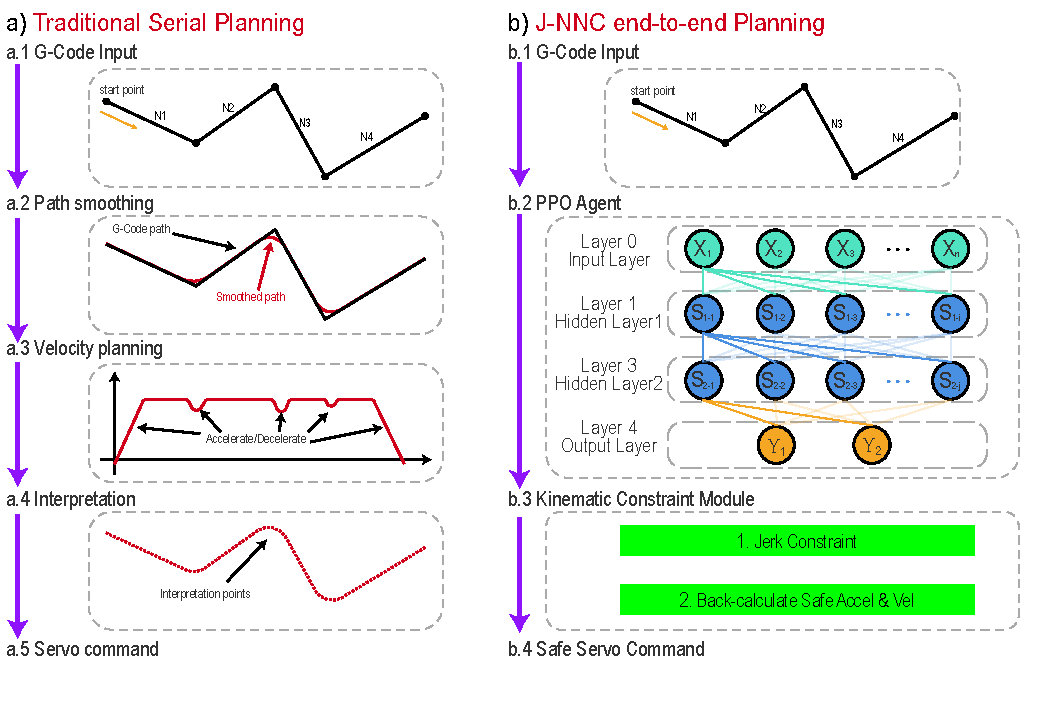
\includegraphics[width=0.9\linewidth]{Figure_1.pdf}
\caption{Comparison of conventional serial motion planning and the J-NNC motion-planning framework. J-NNC denotes the Jerk-constrained Neural Numerical Controller, a neural-network-based CNC motion planner with jerk-constrained action projection.}
\label{fig:comparison_arch}
\end{figure}

The main contributions are as follows:
\begin{enumerate}
\item[(1)] A KCM is developed to project raw steering and feedrate outputs into executable commands while satisfying velocity, acceleration, and jerk limits for both linear and angular motion.
\item[(2)] A tolerance-band one-step decision formulation with Adaptive Preview is proposed to jointly learn trajectory shaping and feedrate regulation from structured geometric and kinematic states.
\item[(3)] Experiments on square, circular, and butterfly-shaped paths show that J-NNC completes the full path and removes the linear-jerk-limit violations observed in the NNC baseline and the no-KCM ablation.
\end{enumerate}

The remainder of this paper is organized as follows. Section 2 defines the problem and models the constraints. Section 3 presents the proposed method. Section 4 reports the experimental settings, comparative results, and ablation analysis. Section 5 concludes the paper.

\section{Problem Formulation}
\label{sec:problem_formulation}
This section defines the motion-planning problem considered in this study, together with the geometric and execution constraints used in the proposed method. These definitions provide the basis for the method described in the following sections.

\subsection{Tool Path and Geometric Feasible Region}
Consider a discrete sequence of cutter-location points generated by a CAM system,
\begin{equation}
P_{\mathrm{raw}}={p_1,p_2,\dots,p_N},
\end{equation}
where $p_i\in\mathbb{R}^2$ denotes a reference point in the interpolation plane. Let $\varepsilon$ denote the prescribed contour tolerance. The reference path is offset by $\varepsilon/2$ on both sides to define the geometric feasible region in which the policy may locally deviate from the reference path:
\begin{equation}
\Omega={x\mid d(x,P_{\mathrm{raw}})\leq \varepsilon/2},
\label{eq:feasible_region}
\end{equation}
where $d(x,P_{\mathrm{raw}})$ denotes the minimum distance from point $x$ to the reference path. This region allows local redistribution of the trajectory within the tolerance band, which helps smooth corner traversal while preserving contour accuracy.

\begin{figure}[htbp]
\centering
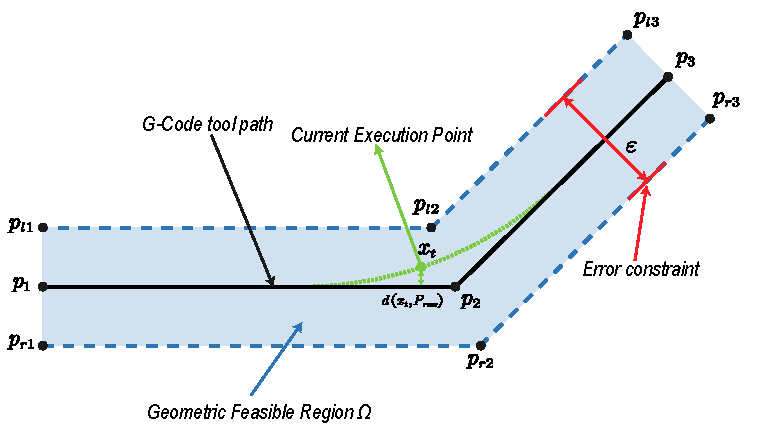
\includegraphics[width=0.9\linewidth]{Figure_2.pdf}
\caption{Geometric feasible region formed by the reference path and the contour tolerance band.}
\label{fig:feasible_region}
\end{figure}

For closed-loop decision making, the reference path is parameterized by arc length. At the current projected arc length $\ell_t$, local geometric quantities are extracted, including the normal error, tangential direction, distance to the next corner, and turning angle of the next corner. These quantities are used in the state representation, reward weighting, and corner-mode identification.

\subsection{Constrained Action Decision Formulation}
At each interpolation period $\Delta t$, the policy receives the current state $s_t$ and outputs a normalized action $a_t^{\pi}$. The kinematic constraint module (KCM) projects this action into an executable control command, which is then applied to the environment. The environment updates the position, orientation, and kinematic state, and returns the immediate reward $r_t$. The task is therefore written as a constrained sequential decision-making problem:
\begin{equation}
\max_{\pi}\ \mathbb{E}{\pi}\left[\sum{t=0}^{T} \gamma^t r_t\right],
\end{equation}
subject to the geometric constraint
\begin{equation}
x_t\in \Omega,
\end{equation}
and the execution-side kinematic constraints
\begin{equation}
|v_t|\leq V_{\max},\quad |a_t|\leq A_{\max},\quad |j_t|\leq J_{\max},
\end{equation}
\begin{equation}
|\omega_t|\leq \Omega_{\max},\quad |\dot{\omega}t|\leq A{\max}^{\omega},\quad |\ddot{\omega}t|\leq J{\max}^{\omega}.
\end{equation}
Here, $v_t$, $a_t$, and $j_t$ denote the linear velocity, linear acceleration, and linear jerk, respectively, whereas $\omega_t$, $\dot{\omega}_t$, and $\ddot{\omega}_t$ denote the angular velocity, angular acceleration, and angular jerk, respectively.

\section{Methodology}
\label{sec:methodology}
\subsection{Overall Framework}
In this paper, Adaptive Preview denotes the state-dependent preview mechanism of J-NNC, whereas look-ahead is retained only when referring to conventional CNC look-ahead interpolation or prior work.

Motion planning for hybrid tool paths is formulated as a closed-loop decision process in a reinforcement learning setting. The policy network acts as the agent, and the tool-path simulation system, which accounts for contour tolerance and kinematic constraints, acts as the environment. At each interpolation cycle, the environment builds the state $s_t$ from the current execution position, kinematic state, local corner information, and Adaptive Preview geometry. Given $s_t$, the policy $\pi_\theta$ produces an action $a_t$ that gives the steering, feedrate, and Adaptive Preview adjustment commands for the current cycle. The action is corrected by the KCM and then applied to the environment. The environment moves to the next state $s_{t+1}$ and returns a reward $r_t$ based on path progress, contour error, and motion smoothness. During training, reward feedback updates the policy parameters, enabling the policy to learn a control law for trajectory smoothing, feedrate planning, and kinematic-constraint satisfaction within the tolerance band.

\figref{fig:framework} shows the overall framework of the proposed method. Given a reference path and a contour tolerance, the environment carries out path projection, corner scanning, and Adaptive Preview geometry extraction to form a structured state vector at the current time step. The policy network outputs a normalized action. The steering and feedrate components are mapped to the pre-projection motion control variables $(\omega^{pre}_t, v^{pre}_t)$, and the Adaptive Preview component is mapped to the current Adaptive Preview distance $L_t$. The KCM then uses the velocity, acceleration, and jerk states from the previous time step to project $(\omega^{pre}_t, v^{pre}_t)$ onto the feasible kinematic set. This projection gives the executable control variables $(\omega_t, v_t)$, which satisfy the velocity, acceleration, and jerk limits. The execution result updates the current position, kinematic quantities, corner phase, and Adaptive Preview observations. During training, the same result also enters the policy update through the reward signal. The whole procedure forms a closed reinforcement learning loop for motion planning.

\begin{figure}[htbp]
\centering
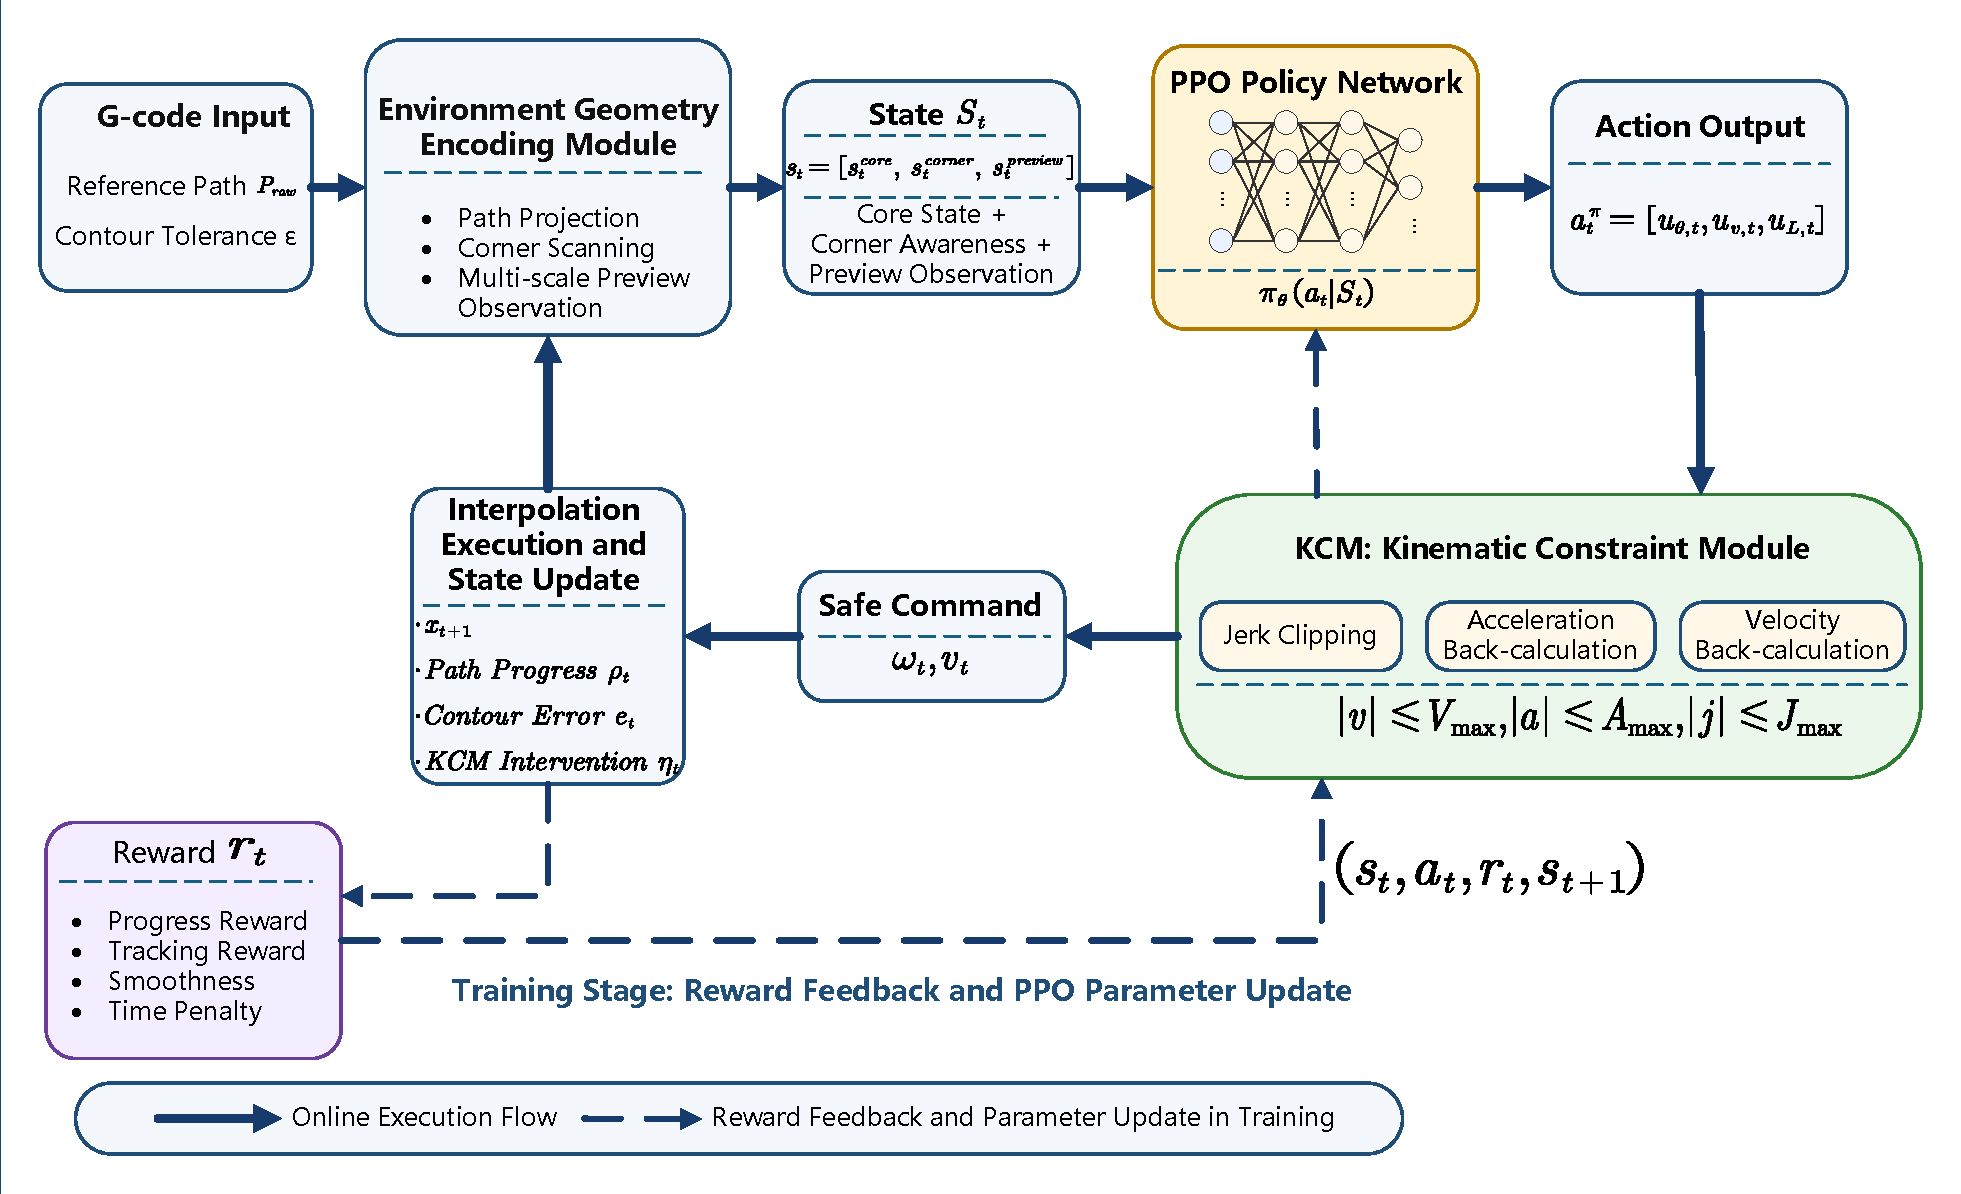
\includegraphics[width=0.9\linewidth]{Figure_3.pdf}
\caption{Overall closed-loop framework of the proposed method.}
\label{fig:framework}
\end{figure}

\subsection{State Design}
A hierarchical structured state representation is used:
\begin{equation}
s_t=[s_t^{core},\ s_t^{corner},\ s_t^{\mathrm{AP}}].
\end{equation}
Here, $s_t^{core}$ describes the local tracking and kinematic state at the current time step, $s_t^{corner}$ describes the relation between the current path segment and the next corner, and $s_t^{\mathrm{AP}}$ records the geometric trend over several Adaptive Preview distances ahead.

The core state is an eight-dimensional vector:
\begin{equation}
s_t^{core}=[\bar e_t,\ \bar e_{n,t},\ \bar\tau_t,\ \bar v_t,\ \bar a_t,\ \bar\omega_t,\ \rho_t,\ \bar d_{c,t}],
\end{equation}
where $\bar e_t$ is the normalized contour error, $\bar e_{n,t}$ is the signed normal error, and $\bar\tau_t$ is the normalized angular error between the current heading and the local tangent direction. The terms $\bar v_t$, $\bar a_t$, and $\bar\omega_t$ are the normalized linear velocity, linear acceleration, and angular velocity, respectively. In addition, $\rho_t\in[0,1]$ gives the overall path progress, and $\bar d_{c,t}$ is the normalized distance to the next corner.

The corner-aware state is a four-dimensional feature vector:
\begin{equation}
s_t^{corner}=[\bar\phi_t,\ \sigma_t,\ m_t,\ \sigma_t\bar e_{n,t}],
\end{equation}
where $\bar\phi_t$ is the normalized turning angle of the next corner, $\sigma_t\in{-1,0,1}$ is the turning sign of the corner, and $m_t\in{0,1}$ indicates whether the current position is within the corner-influence interval. The last term, $\sigma_t\bar e_{n,t}$, encodes the signed positional relation to the inner or outer side of the turn.

For Adaptive Preview observation, several Adaptive Preview scales ${\lambda_k}{k=1}^{N_L}$ are defined along the arc length of the reference path. Let $\ell_t$ be the arc-length coordinate of the projection of the current execution point onto the reference path. The forward observation point for the $k$-th Adaptive Preview scale is
\begin{equation}
q_t^{(k)}=P{\mathrm{raw}}(\ell_t+\lambda_k L_t),\qquad k=1,\dots,N_L,
\end{equation}
where $\lambda_k$ is the scale coefficient and $L_t$ is the base Adaptive Preview distance used in the current cycle. In this formulation, the near-, medium-, and far-range Adaptive Preview points are determined along the arc length of the reference path, rather than from ray intersections along the current execution direction. For each scale, the angular variation of the forward observation point relative to the current tangent direction and the corresponding distance ratio are extracted:
\begin{equation}
s_t^{\mathrm{AP}}=\big[\Delta \theta_t^{(1)},\ \bar d_t^{(1)},\ \dots,\ \Delta \theta_t^{(N_L)},\ \bar d_t^{(N_L)}\big].
\end{equation}
Here, $\Delta \theta_t^{(k)}$ describes the directional change at the $k$-th Adaptive Preview scale, and $\bar d_t^{(k)}$ is the normalized distance from the current position to the corresponding Adaptive Preview point. The main implementation uses three Adaptive Preview scales.

\subsection{Action Space and Kinematic Constraint Module}
At each control cycle, the policy network outputs a normalized action:
\begin{equation}
a_t^{\pi}=[u_{\theta,t},u_{v,t},u_{L,t}],
\end{equation}
where $u_{\theta,t}\in[-1,1]$ is the normalized steering component, $u_{v,t}\in[0,1]$ is the normalized feedrate component, and $u_{L,t}\in[0,1]$ is the Adaptive Preview adjustment component. Given the admissible Adaptive Preview range $[L_{\min},L_{\max}]$, the physical Adaptive Preview distance is mapped as
\begin{equation}
L_t=L_{\min}+u_{L,t}(L_{\max}-L_{\min}).
\end{equation}
The policy output is first converted to pre-projection motion control variables in physical units:
\begin{equation}
\omega_t^{pre}=u_{\theta,t}\Omega_{\max},\qquad v_t^{pre}=u_{v,t}V_{\max}.
\end{equation}
The Adaptive Preview distance $L_t$ is used to compute the local reference direction and Adaptive Preview geometry. The KCM then projects $(\omega_t^{pre},v_t^{pre})$ onto the kinematically feasible set according to the kinematic state at the previous time step. For the linear-velocity channel, let $v_{t-1}$ and $a_{t-1}$ be the linear velocity and linear acceleration in the previous cycle. The pre-projection acceleration is
\begin{equation}
a_t^{pre}=\frac{v_t^{pre}-v_{t-1}}{\Delta t},
\end{equation}
and the corresponding pre-projection jerk is
\begin{equation}
j_t^{pre}=\frac{a_t^{pre}-a_{t-1}}{\Delta t}.
\end{equation}
The KCM clips this jerk by the jerk bound:
\begin{equation}
j_t=\mathrm{clip}(j_t^{pre},-J_{\max},J_{\max}),
\end{equation}
and then reconstructs the realizable acceleration and velocity for the current cycle:
\begin{equation}
a_t=\mathrm{clip}(a_{t-1}+j_t\Delta t,-A_{\max},A_{\max}),
\end{equation}
\begin{equation}
v_t=\mathrm{clip}\left(v_{t-1}+a_{t-1}\Delta t+\frac{1}{2}j_t\Delta t^2,0,V_{\max}\right).
\end{equation}
The angular-velocity channel uses the same projection procedure. The resulting $(\omega_t,v_t)$ is then applied to the environment as the executable control input. The resulting online projection procedure is summarized in Algorithm~\ref{alg:kcm_projection}.

\begin{algorithm}[H]
\caption{KCM-constrained action projection}
\label{alg:kcm_projection}
\begin{algorithmic}[1]
\Require Policy output $a_t^{\pi}=[u_{\theta,t},u_{v,t},u_{L,t}]$; previous-step kinematic state $(v_{t-1},a_{t-1},\omega_{t-1},\alpha_{t-1})$
\Ensure Executed control variables $(\omega_t,v_t)$ and the updated kinematic state
\State Map $u_{\theta,t}$ and $u_{v,t}$ to the unconstrained motion commands $(\omega_t^{pre},v_t^{pre})$
\State Map $u_{L,t}$ to the Adaptive Preview distance $L_t$
\State Compute the unconstrained linear acceleration $a_t^{pre}$ from $v_t^{pre}$ and $v_{t-1}$
\State Compute the unconstrained linear jerk $j_t^{pre}$ from $a_t^{pre}$ and $a_{t-1}$
\State Clip $j_t^{pre}$ to obtain $j_t$ under the prescribed jerk bound
\State Recover the linear acceleration $a_t$ from $j_t$ and apply acceleration clipping
\State Integrate $(v_{t-1},a_{t-1},j_t)$ to obtain the linear velocity $v_t$ for the current control cycle
\State Apply the same procedure to the angular-velocity channel to obtain the constrained angular velocity $\omega_t$
\State Return the executed control variables $(\omega_t,v_t)$ and the updated kinematic state
\end{algorithmic}
\end{algorithm}

The intervention degree of the KCM is defined as
\begin{equation}
\eta_t=\frac{|v_t-v_t^{pre}|}{V_{\max}}+\frac{|\omega_t-\omega_t^{pre}|}{\Omega_{\max}}.
\end{equation}
This scalar is not part of the primary optimization objective. It is used only as an auxiliary metric in the result analysis.

\subsection{Reward Design}
The instantaneous reward is
\begin{equation}
r_t=r_t^{prog}+r_t^{track}+r_t^{dir}+r_t^{smooth}.
\label{eq:reward_total}
\end{equation}

The progress reward is defined as
\begin{equation}
r_t^{prog}=w_p\max(0,\rho_t-\rho_{t-1}),
\end{equation}
where $\rho_t$ is the overall path progress.

The contour-error penalty is defined as
\begin{equation}
\phi_e(e_t)=
\begin{cases}
0, & |e_{n,t}|\leq \delta_t,\\[4pt]
\left(\dfrac{|e_{n,t}|-\delta_t}{\varepsilon/2}\right)^2, & |e_{n,t}|>\delta_t,
\end{cases}
\end{equation}
and the corresponding tracking reward is
\begin{equation}
r_t^{track}=-w_e(c_t)\phi_e(e_t).
\end{equation}
Here, $\delta_t$ is the relaxed boundary within the tolerance band, and $c_t\in[0,1]$ is the local corner intensity. They are defined as
\begin{equation}
\delta_t=\kappa_{\delta}\frac{\varepsilon}{2}\mathbf{1}(m_t=1),
\end{equation}
\begin{equation}
c_t=\mathrm{clip}\left((1-\alpha_c)c_{t-1}+\alpha_c\frac{|\Delta\theta_t^{(N_L)}|}{\theta_0},0,1\right),
\end{equation}
where $\kappa_{\delta}$ is the error-relaxation ratio, $m_t$ indicates whether the current state is within the corner-influence region, $\Delta\theta_t^{(N_L)}$ is the Adaptive Preview directional change at the farthest scale, $\theta_0$ is the normalization angle for local corner intensity, and $\alpha_c=1/T_c$ is the exponential moving-average coefficient. In the main experiments, $\kappa_{\delta}$ is set to $0$. Thus, the contour-error term has no additional dead zone, while $c_t$ is still used to adjust the tracking and smoothness weights.

The directional consistency term is defined as
\begin{equation}
r_t^{dir}=-w_{\tau}|\tau_t|,
\end{equation}
where $\tau_t$ is the angular error between the current heading and the local reference direction.

The smoothness term is defined as
\begin{equation}
r_t^{smooth}=-w_s(c_t)\psi_t,
\end{equation}
where $\psi_t$ can be a normalized measure of linear jerk, angular acceleration, or angular jerk. The weight $w_s(c_t)$ is adjusted according to the local corner intensity. One implementation is
\begin{equation}
w_s(c_t)=w_s^0 c_t^{\gamma}, \qquad \gamma>1,
\end{equation}
where $w_s(c_t)$ increases with $c_t$.

\subsection{PPO Training Configuration}
\label{sec:ppo_training_configuration}
The policy is trained with Proximal Policy Optimization (PPO). The Actor is a shared multilayer perceptron with three hidden layers of widths $256$, $128$, and $64$. Each layer uses ELU activation followed by LayerNorm. Separate output heads parameterize the mean and standard deviation of a three-dimensional action distribution. The steering mean is mapped to $[-1,1]$ with $\tanh$, while the feedrate and Adaptive Preview mean are mapped to $[0,1]$ with the sigmoid function. The standard deviation is obtained by applying the softplus function and then adding $10^{-3}$ for numerical stability. The Critic has layer widths $256,128,64,1$ and uses ELU activation, LayerNorm, and a dropout rate of $0.1$. The main training hyperparameters are listed in \tabref{tab:ppo_params}.

\begin{table}[H]
\centering
\caption{PPO hyperparameters and training protocol.}
\label{tab:ppo_params}
\small
\begin{tabular}{lp{0.68\textwidth}}
\toprule
\textbf{Parameter} & \textbf{Value}\\
\midrule
Actor learning rate & $3.0\times10^{-4}$\\
Critic learning rate & $1.5\times10^{-4}$\\
Discount factor $\gamma$ & $0.99$\\
GAE parameter $\lambda$ & $0.95$\\
PPO clip coefficient & $0.1$\\
Number of epochs per update & $8$\\
Entropy coefficient & $0.01$\\
Gradient clipping & $0.5$\\
\bottomrule
\end{tabular}
\end{table}


\section{Experiments and Results}
\label{sec:experiments_results}

We evaluate J-NNC in simulation on three paths with different geometric demands. The tests focus on three practical requirements of CNC interpolation: the tool should reach the end of the commanded path, local transitions should remain within the contour-tolerance band, and the executed commands should satisfy the prescribed velocity, acceleration, and jerk limits. The main comparison uses the neural-network numerical control (NNC) baseline and a traditional two-step baseline. The ablation study then examines Adaptive Preview, KCM, Adaptive Preview observation, and reward scheduling.

\subsection{Experimental Settings}

The three test paths are selected to stress different parts of the planner. The square path emphasizes sharp-corner deceleration, turning, and re-acceleration. The circular path tests continuous turning under sustained contour control. The butterfly-shaped path contains mixed curvature changes and local geometric variation.

Unless otherwise stated, the J-NNC and ablation evaluations use a contour-tolerance band of $\varepsilon=2.5$ mm, an interpolation period of $\Delta t=0.001$ s, and a maximum episode length of $60000$ steps, corresponding to $60$ s. The linear kinematic limits are $V_{\max}=100$ mm/s, $A_{\max}=2000$ mm/s$^2$, and $J_{\max}=62500$ mm/s$^3$. The Adaptive Preview distance is selected within $[0.8,4.6]$ mm, and the multi-scale observation uses scales $(0.5,1.0,2.0)$ with $8$ forward points.

The main comparison includes J-NNC and two baselines. The NNC baseline directly executes the learned policy output, following Li et al.~\cite{Li2020}. The traditional two-step baseline smooths the path first and then applies jerk-limited feedrate scheduling. We report contour error, linear-jerk exceedance, elapsed interpolation time, and dynamic-limit use.

Each ablation modifies one part of the proposed method. The fixed Adaptive Preview setting replaces the state-dependent Adaptive Preview action with a fixed Adaptive Preview distance. The no-KCM setting removes the execution-layer kinematic-constraint projection and directly applies the policy output in the environment. The setting without Adaptive Preview observation removes the multi-scale forward geometric input. The no-dual-reward setting disables the separate reward scheduling for straight and corner segments. These variants separate the effects of Adaptive Preview, execution-side constraints, forward geometric information, and reward structure.

Because the task is constrained CNC motion planning, a shorter execution time is useful only when both contour and jerk constraints are satisfied.

\subsection{Main Comparative Results}

This subsection reports the comparative results of J-NNC, the NNC baseline, and a traditional two-step baseline on three representative paths. The traditional two-step baseline follows the conventional serial pipeline: a fixed corner-smoothed path is first generated from the reference path, and conservative jerk-limited feedrate scheduling is then performed along that fixed path, following the smooth-then-schedule strategy used in local corner smoothing methods~\cite{Sencer2014}. The comparison between J-NNC and the NNC baseline mainly evaluates the role of explicit execution-layer kinematic projection for learned direct control, whereas the comparison between J-NNC and the traditional two-step baseline evaluates whether closed-loop one-step tolerance-band planning can improve efficiency and dynamic-limit use compared with a serial smooth-then-schedule pipeline.

\begin{table}[H]
\centering
\caption{Performance on representative test paths for the NNC baseline, the traditional two-step baseline, and J-NNC.}
\label{tab:main_results}
\resizebox{0.98\textwidth}{!}{
\begin{tabular}{llccc}
\toprule
\textbf{Path} & \textbf{Measure} & \textbf{NNC baseline} & \textbf{Traditional two-step} & \textbf{J-NNC}\\
\midrule
\multirow{3}{*}{square} & Peak contour error [mm] & 0.676 & 0.309 & 0.834\\
& Peak relative exceedance of the linear-jerk limit & 3199.000 & 0.000 & 0.000\\
& Elapsed interpolation time [s] & 8.672 & 24.780 & 12.192\\
\midrule
\multirow{3}{*}{circle} & Peak contour error [mm] & 6.259 & 0.000 & 0.096\\
& Peak relative exceedance of the linear-jerk limit & 3199.000 & 0.000 & 0.000\\
& Elapsed interpolation time [s] & 60.000 & 17.499 & 9.117\\
\midrule
\multirow{3}{*}{butterfly} & Peak contour error [mm] & 0.207 & 0.012 & 0.745\\
& Peak relative exceedance of the linear-jerk limit & 3199.000 & 0.000 & 0.000\\
& Elapsed interpolation time [s] & 5.807 & 15.360 & 10.480\\
\bottomrule
\end{tabular}
}
\end{table}

\begin{table}[H]
\centering
\caption{Efficiency and dynamic-limit use for J-NNC and the traditional two-step baseline.}
\label{tab:efficiency_utilization}
\resizebox{0.98\textwidth}{!}{
\begin{tabular}{llcccc}
\toprule
\textbf{Path} & \textbf{Method} & \textbf{Mean feedrate use} & \textbf{95th-percentile acceleration use} & \textbf{95th-percentile linear-jerk use} & \textbf{Active jerk-limit engagement rate}\\
\midrule
\multirow{2}{*}{square} & Traditional two-step & 0.161 & 0.000 & 0.000 & 0.000\\
& J-NNC & 0.328 & 0.562 & 1.000 & 0.991\\
\midrule
\multirow{2}{*}{circle} & Traditional two-step & 0.180 & 0.000 & 0.000 & 0.000\\
& J-NNC & 0.345 & 0.562 & 1.000 & 0.999\\
\midrule
\multirow{2}{*}{butterfly} & Traditional two-step & 0.150 & 0.039 & 0.250 & 0.000\\
& J-NNC & 0.221 & 0.531 & 1.000 & 0.988\\
\bottomrule
\end{tabular}
}
\end{table}

\tabref{tab:main_results} reports the three core comparison measures: peak contour error, peak relative exceedance of the linear-jerk limit, and elapsed interpolation time. \tabref{tab:efficiency_utilization} then isolates how the traditional two-step baseline and J-NNC use the available feedrate, acceleration, and jerk-limit margins. Mean feedrate use reflects the average use of the commanded feedrate limit. The 95th-percentile acceleration use indicates whether the acceleration constraint is substantially invoked. The active jerk-limit engagement rate measures how often the trajectory operates near the jerk limit during active acceleration phases. This metric is meaningful only when the corresponding jerk exceedance remains zero.

The comparison with NNC mainly highlights dynamic feasibility. Although NNC gives shorter times on the square and butterfly paths, those times arise from unconstrained direct policy outputs with severe linear-jerk exceedance. The shorter NNC time is not physically meaningful because the executed command violates the prescribed jerk constraint. J-NNC instead keeps the peak relative exceedance of the linear-jerk limit at zero on all three paths and also reduces the circular-path peak contour error substantially relative to NNC.

Compared with the traditional two-step baseline, J-NNC mainly improves efficiency under the same jerk-feasibility requirement. Both methods satisfy the jerk constraint, but J-NNC reduces the elapsed interpolation time from $24.780$ s to $12.192$ s on the square path, from $17.499$ s to $9.117$ s on the circular path, and from $15.360$ s to $10.480$ s on the butterfly path. The dynamic-limit use measures in \tabref{tab:efficiency_utilization} explain this difference: J-NNC has higher mean feedrate use and operates near the jerk limit more frequently during active acceleration phases, whereas the two-step baseline remains conservative after the geometric smoothing stage. This indicates that the proposed closed-loop planner uses the tolerance band and the kinematic limits jointly, instead of fixing the geometry first and then scheduling a cautious feedrate along that fixed curve.

\begin{figure}[!htbp]
\centering
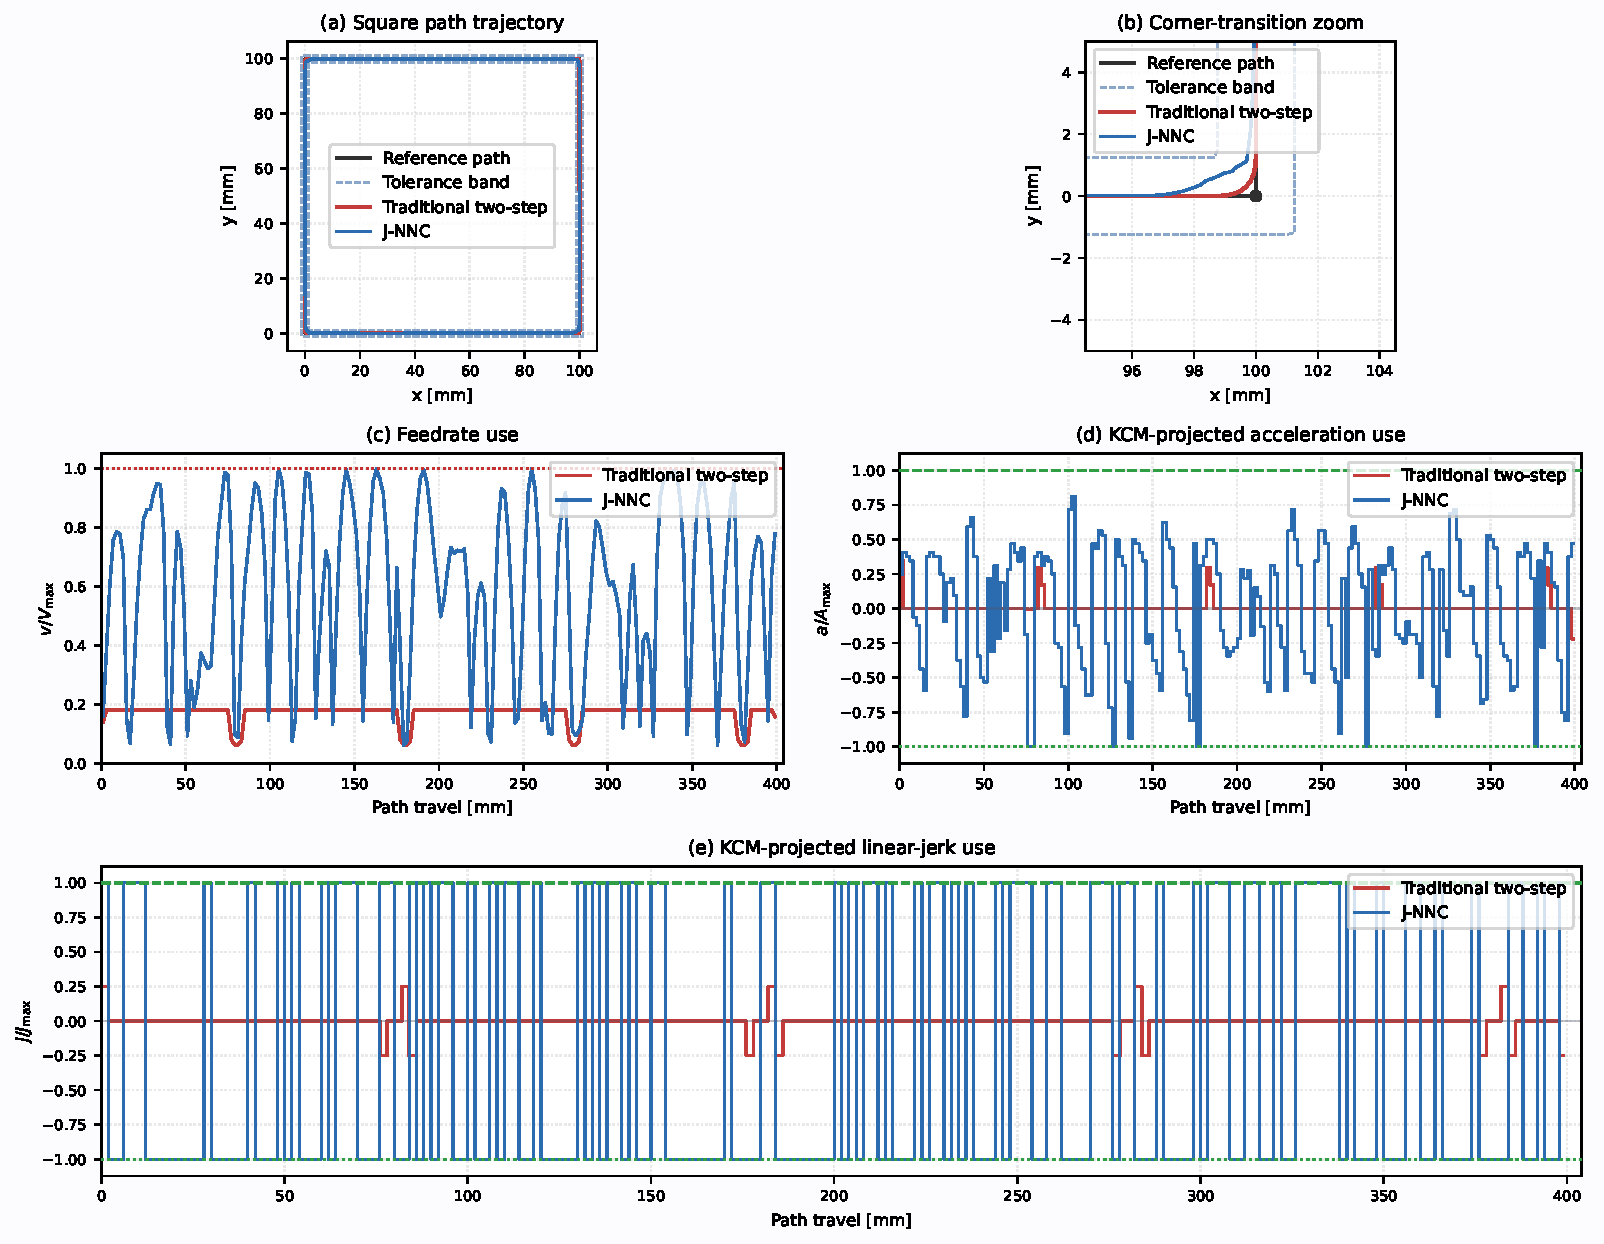
\includegraphics[width=0.98\linewidth]{Figure_4.pdf}
\caption{Square-path comparison between J-NNC and the traditional two-step baseline: (a) square path trajectory; (b) corner-transition zoom; (c) path-travel-aligned feedrate use $v/V_{\max}$; (d) path-travel-aligned KCM-projected signed acceleration use $a/A_{\max}$; (e) path-travel-aligned KCM-projected signed linear-jerk use $j/J_{\max}$.}
\label{fig:two_step_comparison}
\end{figure}


\figref{fig:two_step_comparison} illustrates this difference on the square path. J-NNC starts the corner transition earlier within the tolerance band and maintains higher path-travel-aligned feedrate use, while the KCM-projected signed acceleration and signed linear jerk remain within the prescribed bounds. The two-step baseline also stays feasible, but its feedrate, acceleration, and jerk-limit use are lower, which explains the longer elapsed interpolation time reported in \tabref{tab:main_results}.

\figref{fig:qualitative_results} presents the trajectory comparisons on the three paths.

\begin{figure}[!htbp]
\centering
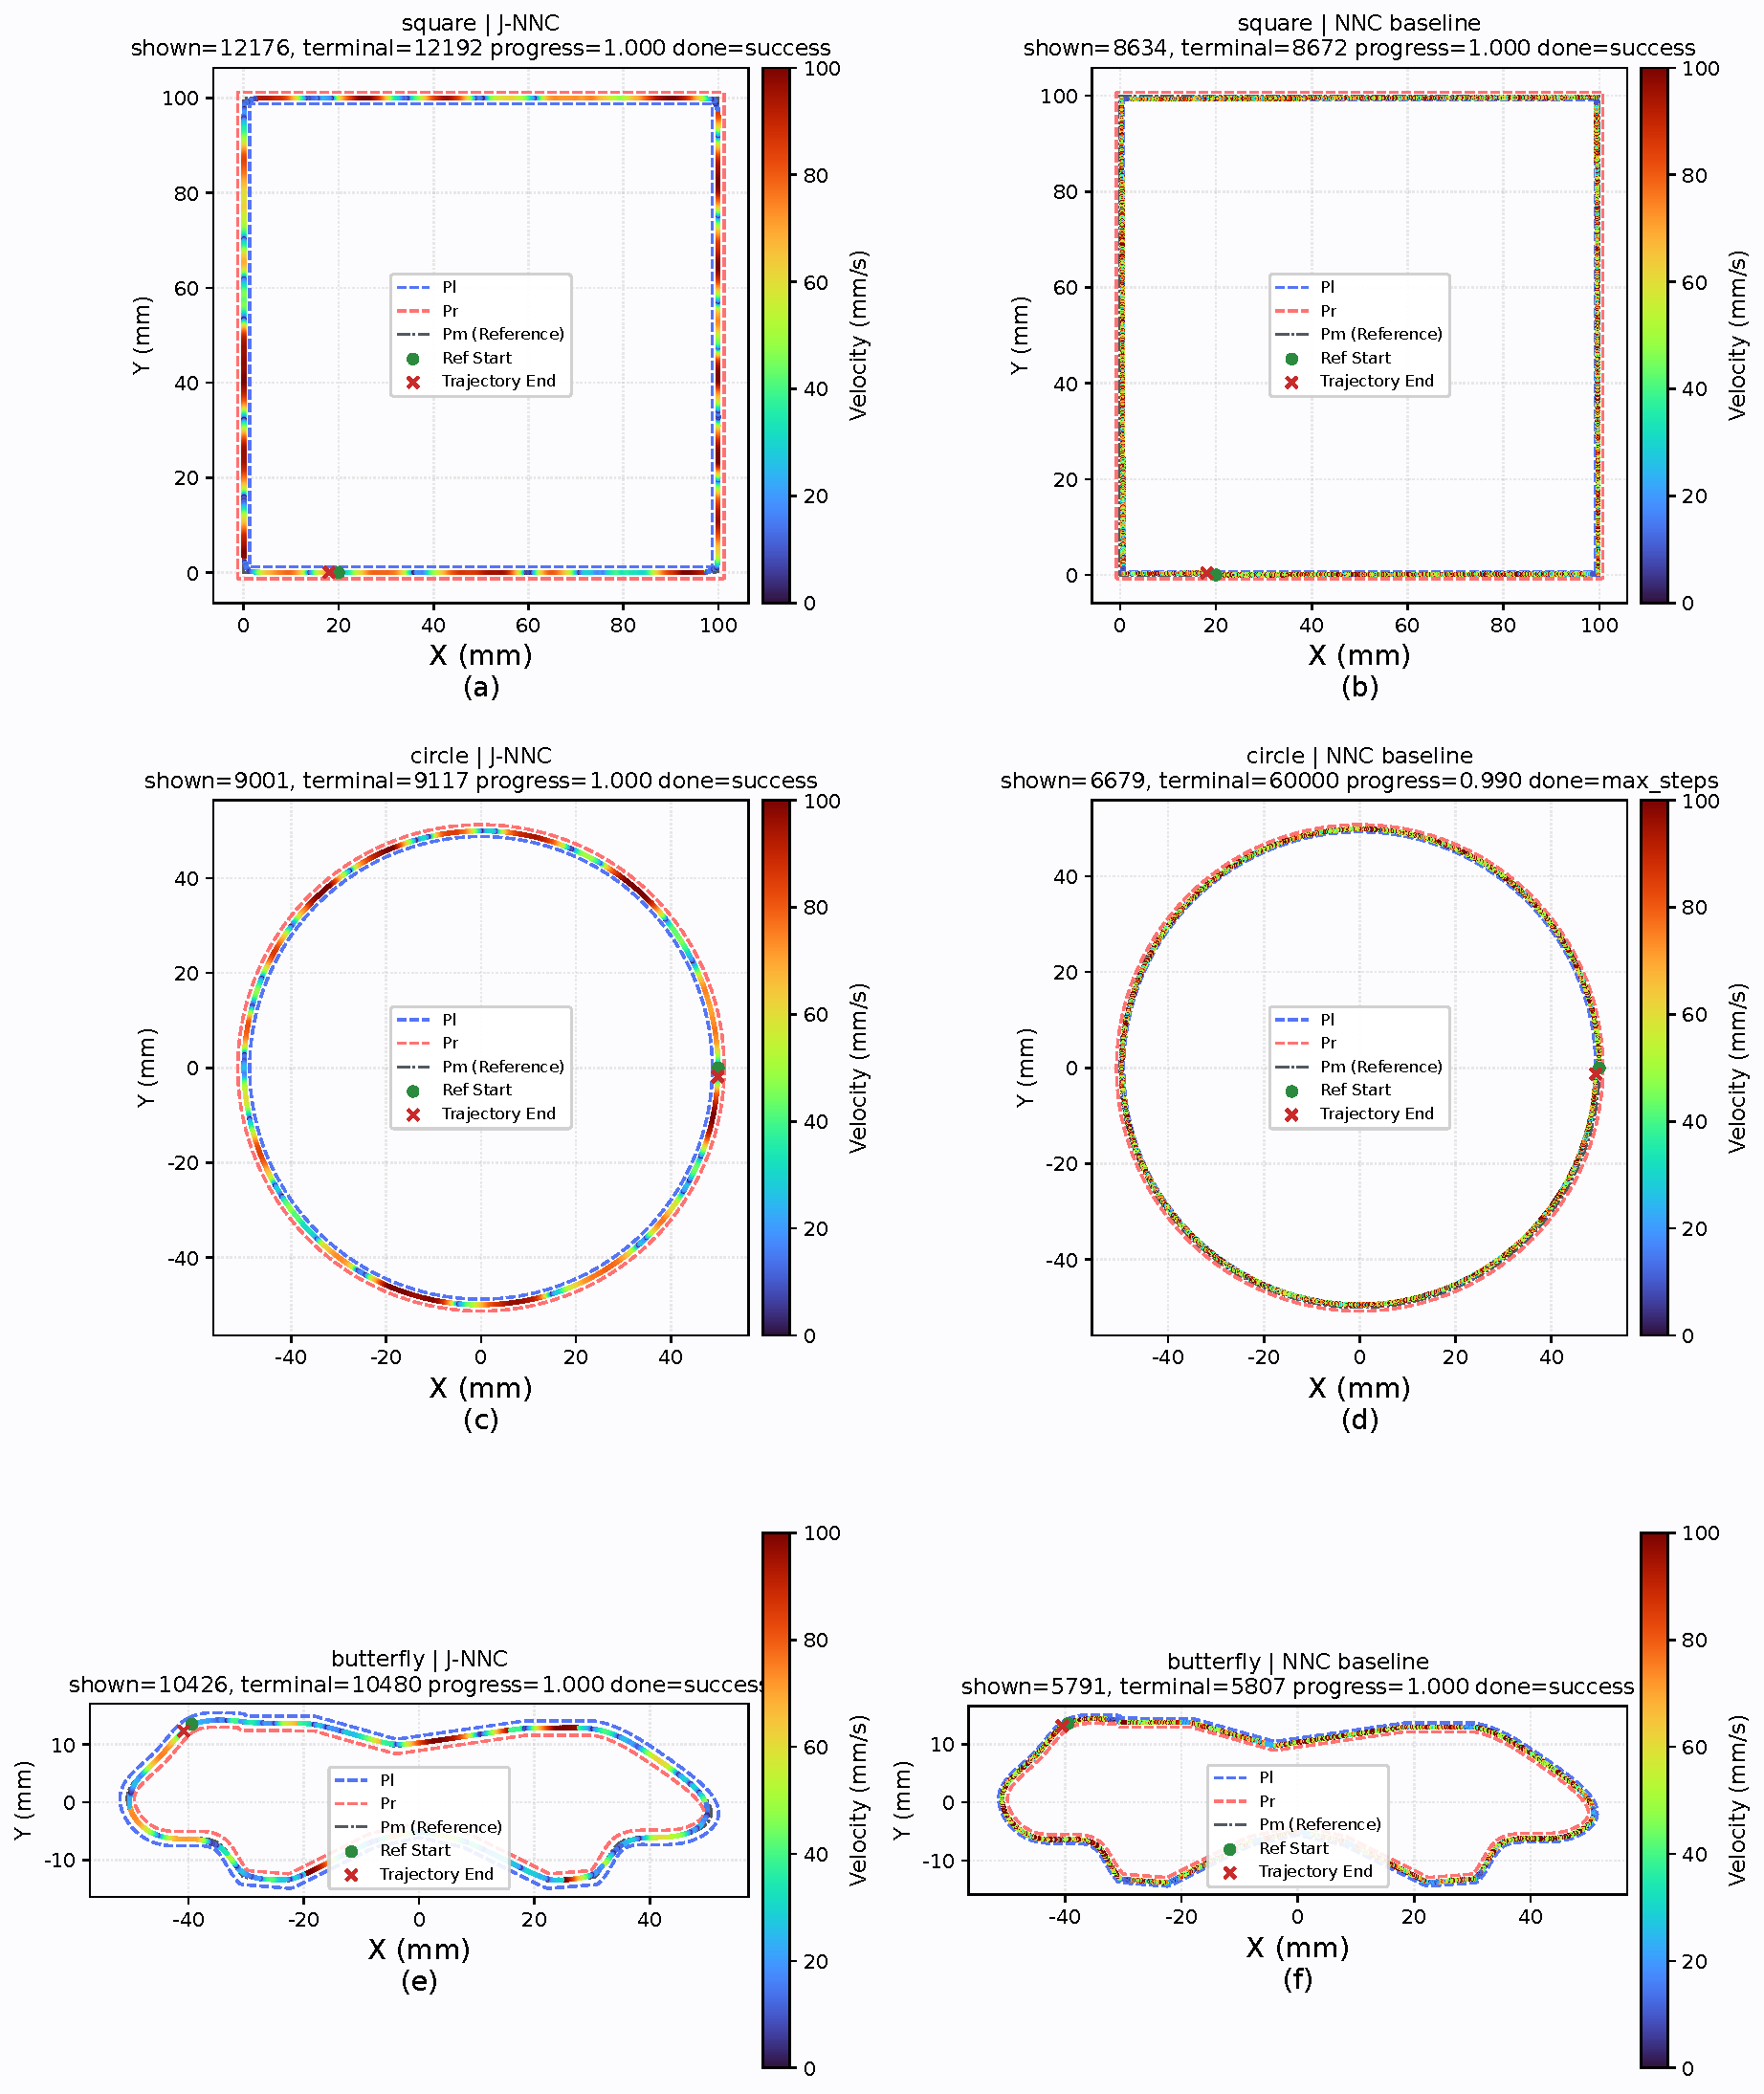
\includegraphics[width=0.96\linewidth]{Figure_5.pdf}
\caption{Trajectory comparison between J-NNC and the NNC baseline on representative paths: (a) square path, J-NNC; (b) square path, NNC baseline; (c) circular path, J-NNC; (d) circular path, NNC baseline; (e) butterfly-shaped path, J-NNC; (f) butterfly-shaped path, NNC baseline.}
\label{fig:qualitative_results}
\end{figure}


In \figref{fig:qualitative_results}(a)--(f), the J-NNC trajectories stay within the tolerance band but do not simply follow the reference polyline. On the square path, J-NNC forms local corner transitions, whereas NNC stays closer to the original polyline. On the circular path, J-NNC advances continuously with small contour error, whereas NNC does not complete the path. On the butterfly-shaped path, J-NNC introduces moderate offsets in regions where the curvature changes. These path-level results show how the tolerance band is used as controllable geometric freedom, and the square-corner region provides a clearer view of this behavior.

\begin{figure}[!htbp]
\centering
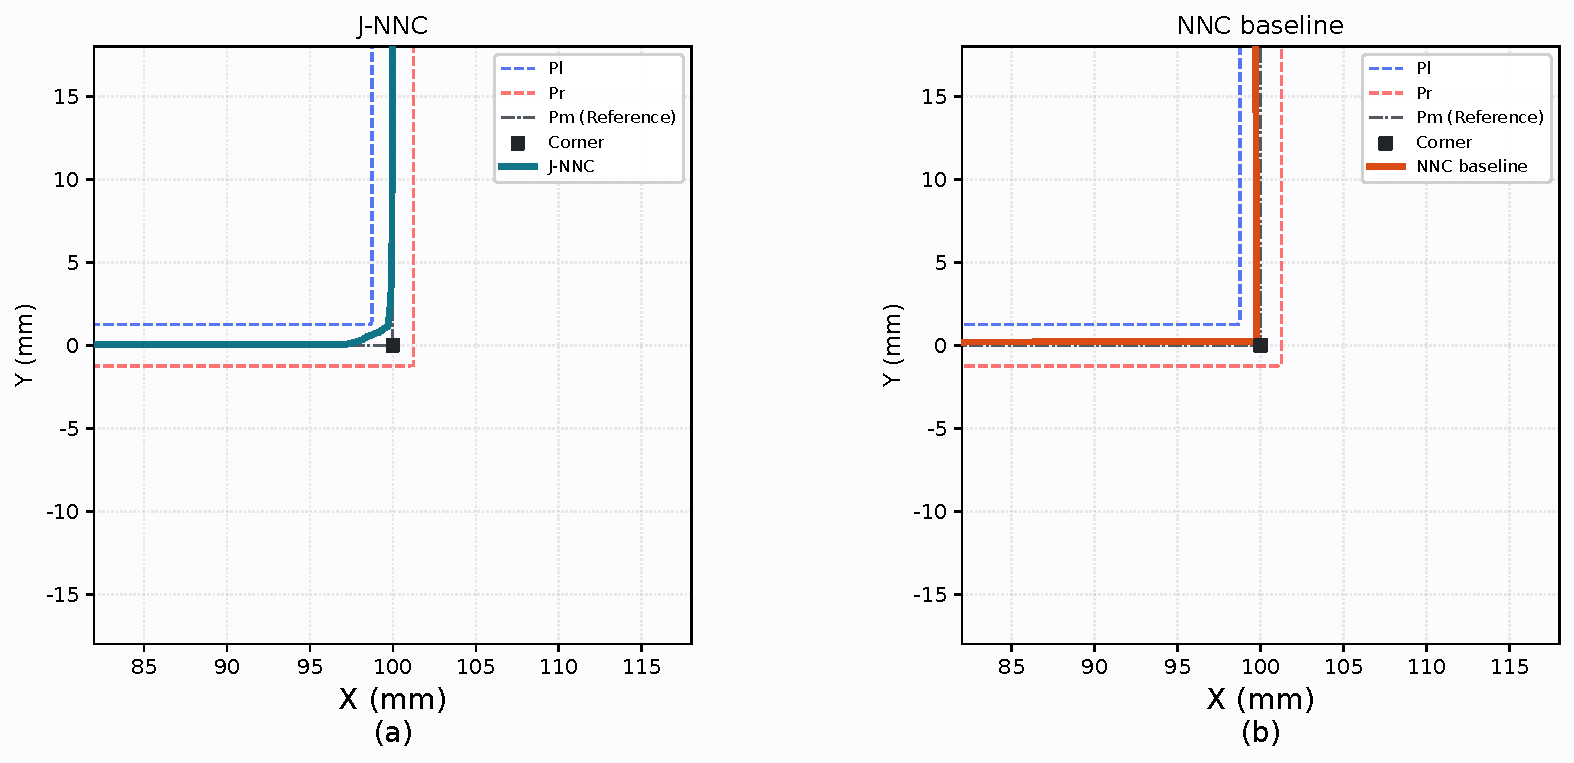
\includegraphics[width=0.82\linewidth]{Figure_6.pdf}
\caption{Local zoomed-in comparison in the square-corner region: (a) J-NNC; (b) NNC baseline.}
\label{fig:square_corner_zoom}
\end{figure}


\figref{fig:square_corner_zoom} shows that J-NNC begins the directional transition before reaching the vertex and distributes the turn inside the tolerance band. The NNC baseline remains closer to the two reference segments, so the change in direction is concentrated around the corner. This local behavior explains why the NNC trajectory can appear geometrically close to the polyline while still producing severe jerk-limit violations in \tabref{tab:main_results}. In contrast, J-NNC uses the admissible geometric margin to smooth the corner and then projects the learned command onto the feasible kinematic set, so the local transition remains executable.

\Needspace{12\baselineskip}

Taken together, these comparisons separate the two advantages of J-NNC. Relative to NNC, it preserves learned path advancement while making the commands executable under the jerk bound; the corner zoom in \figref{fig:square_corner_zoom} shows the local geometric mechanism behind this improvement. Relative to the traditional two-step baseline, it uses the tolerance band and the jerk limit more actively, shortening execution time without relaxing jerk feasibility.

\subsection{Ablation Results}

The ablation study modifies Adaptive Preview, KCM, Adaptive Preview observation, and the straight-line/corner dual-reward scheme. \tabref{tab:ablation} reports the outcome, final progress, peak contour error, peak relative exceedance of the linear-jerk limit, and elapsed time for each path and configuration.

\begin{table}[H]
\centering
\caption{Path-level results of the structured ablation study.}
\label{tab:ablation}
\begingroup
\small
\setlength{\tabcolsep}{3pt}
\renewcommand{\arraystretch}{1.16}
\resizebox{0.98\textwidth}{!}{%
\begin{tabular}{>{\raggedright\arraybackslash}p{0.23\textwidth}lccccc}
\toprule
\textbf{Configuration} & \textbf{Path} & \textbf{Outcome} & \textbf{Final progress} & \begin{tabular}[c]{@{}c@{}}\textbf{Peak contour}\\\textbf{error [mm]}\end{tabular} & \begin{tabular}[c]{@{}c@{}}\textbf{Peak jerk-limit}\\\textbf{exceedance}\end{tabular} & \textbf{Elapsed time [s]}\\
\midrule
\multirow{3}{0.23\textwidth}{J-NNC} & square & success & 1.000 & 0.834 & 0.000 & 12.192\\
& circle & success & 1.000 & 0.096 & 0.000 & 9.117\\
& butterfly & success & 1.000 & 0.745 & 0.000 & 10.480\\
\addlinespace[0.35em]
\multirow{3}{0.23\textwidth}{Fixed Adaptive Preview} & square & success & 1.000 & 0.699 & 0.000 & 8.680\\
& circle & success & 1.000 & 0.046 & 0.000 & 4.804\\
& butterfly & success & 1.000 & 0.638 & 0.000 & 5.049\\
\addlinespace[0.35em]
\multirow{3}{0.23\textwidth}{Without KCM} & square & success & 1.000 & 0.722 & 3199.000 & 10.301\\
& circle & success & 1.000 & 0.061 & 3199.000 & 5.926\\
& butterfly & success & 1.000 & 0.707 & 3199.000 & 7.446\\
\addlinespace[0.35em]
\multirow{3}{0.23\textwidth}{Without Adaptive Preview observation} & square & success & 1.000 & 0.805 & 0.000 & 8.151\\
& circle & success & 1.000 & 0.077 & 0.000 & 4.573\\
& butterfly & success & 1.000 & 0.820 & 0.000 & 6.044\\
\addlinespace[0.35em]
\multirow{3}{0.23\textwidth}{Without straight-line/corner dual rewards} & square & success & 1.000 & 0.824 & 0.000 & 15.132\\
& circle & success & 1.000 & 0.030 & 0.000 & 10.388\\
& butterfly & success & 1.000 & 0.918 & 0.000 & 9.623\\
\bottomrule
\end{tabular}
}
\endgroup
\end{table}

\tabref{tab:ablation} shows that all ablated configurations complete the evaluated trajectories, but they differ in elapsed time, contour error, and jerk feasibility. The no-KCM setting isolates the role of execution-layer projection. Without this projection, the controller still advances along the paths, but the jerk violation increases sharply. Because KCM is active in all other configurations, their peak relative exceedance of the linear-jerk limit remains zero.

\figref{fig:jerk_constraint_comparison} compares the linear jerk of J-NNC with that of the configuration without KCM on the same representative path.

\begin{figure}[htbp]
\centering
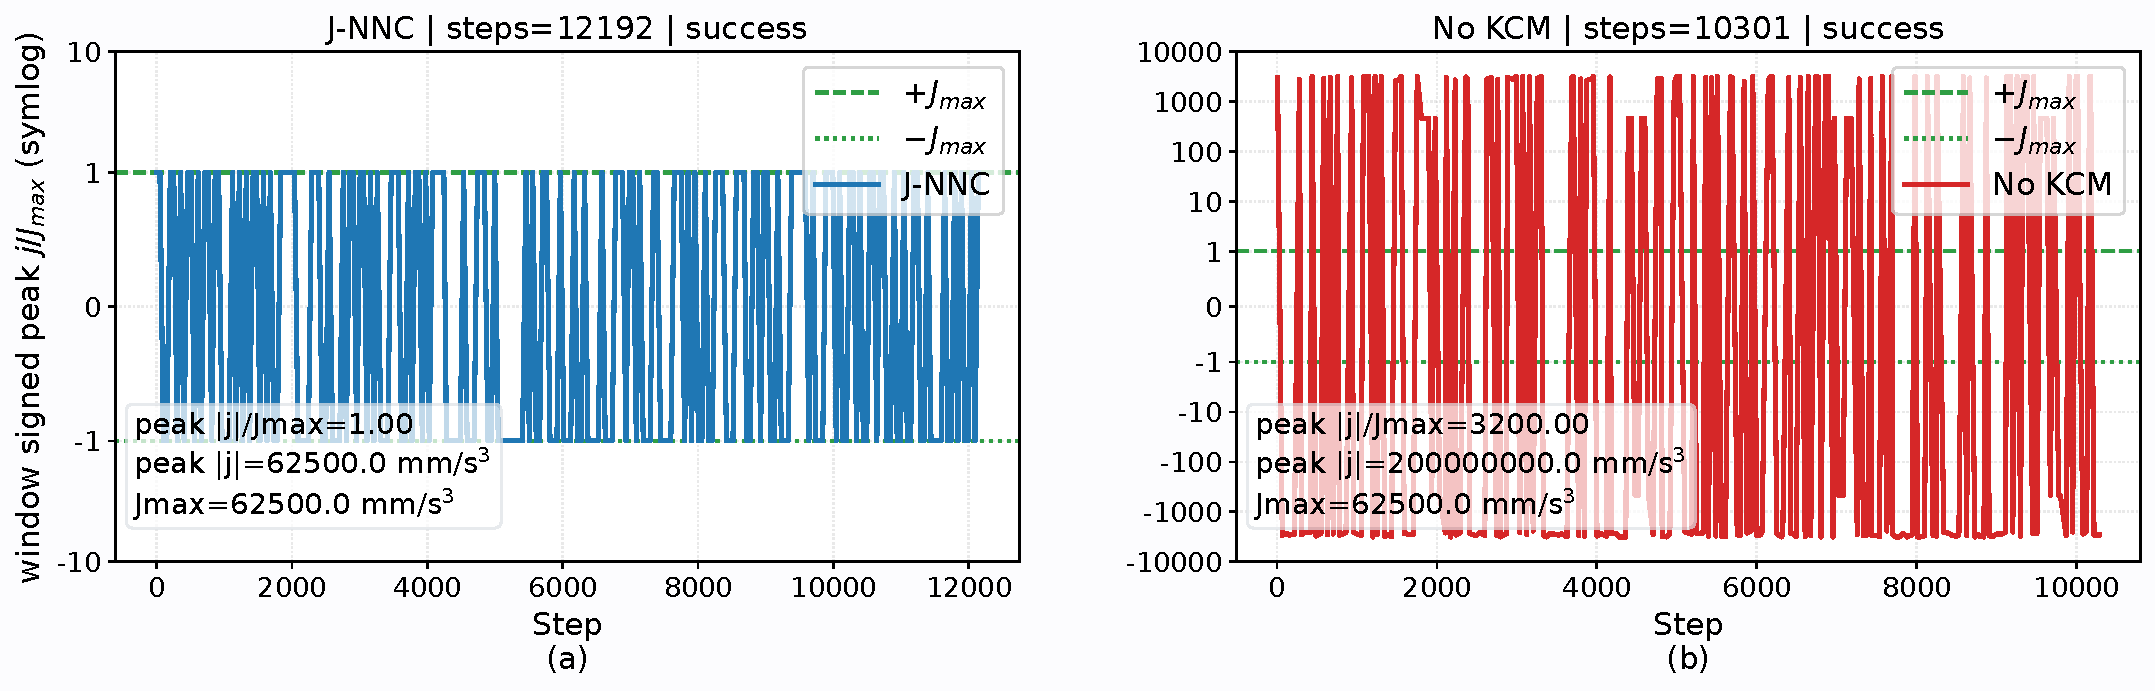
\includegraphics[width=0.96\linewidth]{Figure_7.pdf}
\caption{Linear-jerk constraint comparison on the same representative path: (a) J-NNC with KCM; (b) ablated configuration without KCM.}
\label{fig:jerk_constraint_comparison}
\end{figure}


As shown in \figref{fig:jerk_constraint_comparison}(a), the linear jerk of J-NNC stays within the bound defined by $J_{\max}$. In \figref{fig:jerk_constraint_comparison}(b), removing KCM produces high-amplitude jerk spikes. This result confirms that faster traversal or smaller contour error alone is insufficient for CNC interpolation; the learned command must also be projected onto the feasible kinematic set.

The remaining ablations give a more nuanced view of Adaptive Preview and reward design. The fixed Adaptive Preview setting is feasible and, in the reported runs, can be faster than the state-dependent setting. This result does not weaken the role of KCM, but it indicates that the present Adaptive Preview parameterization has not yet fully converted state-dependent Adaptive Preview selection into a consistent speed advantage. Its value is that the policy can vary the forward geometric range according to the local state; the benefit of this design should become clearer with improved parameterization and more diverse paths. Removing Adaptive Preview observation still leaves enough local tracking and corner information to finish the paths, but it reduces access to upcoming geometric trends that can support earlier steering and speed adjustment. Removing the straight-line/corner dual-reward scheme changes the balance among progress, contour regulation, and smoothness, because straight feeding and corner transition require different control priorities.

Overall, the ablation results separate the roles of the main components. KCM is the component that guarantees dynamic feasibility. Adaptive Preview and phase-dependent rewards affect how the feasible commands are selected within the tolerance band, although the current Adaptive Preview design still needs refinement to provide a more consistent advantage over fixed settings. Future improvements should therefore focus on Adaptive Preview parameterization and velocity continuity after corner traversal rather than on relaxing the execution-side jerk projection.

\section{Conclusion}
\label{sec:conclusion}

This paper presented J-NNC, a reinforcement learning-based CNC motion-planning method for mixed CAM-generated tool paths subject to contour-tolerance and kinematic constraints. The main difficulty considered in this work is that geometric smoothing, feedrate planning, and dynamic feasibility cannot be treated independently in practical CNC interpolation. A trajectory that stays close to the reference polyline may still contain sharp direction changes near corners, while a learned controller that advances the path efficiently may produce commands that exceed velocity, acceleration, or jerk limits. J-NNC addresses this issue by treating CNC interpolation as a closed-loop constrained decision-making process, rather than as a serial procedure with separate smoothing and feedrate-planning stages. The structured state and Adaptive Preview action allow the policy to combine tracking, kinematic, corner, and forward-geometric information when planning local transitions within the tolerance band. The KCM further projects learned steering and feedrate outputs into executable commands satisfying velocity, acceleration, and jerk limits. Experiments on square, circular, and butterfly-shaped paths show full path progress and zero maximum relative linear-jerk violation, confirming the importance of explicit action projection compared with the NNC baseline and the no-KCM ablation.

Future work will refine the Adaptive Preview action and corner-phase representation to improve traversal efficiency and velocity continuity after corner transitions. Further validation will include servo lag, axis-level constraints, and real machining experiments to assess practical deployment on CNC systems.

\clearpage
\bibliographystyle{unsrt}
\bibliography{references}

\end{document}
